% Options for packages loaded elsewhere
\PassOptionsToPackage{unicode}{hyperref}
\PassOptionsToPackage{hyphens}{url}
%
\documentclass[
  11pt,
]{article}
\usepackage{amsmath,amssymb}
\usepackage{iftex}
\ifPDFTeX
  \usepackage[T1]{fontenc}
  \usepackage[utf8]{inputenc}
  \usepackage{textcomp} % provide euro and other symbols
\else % if luatex or xetex
  \usepackage{unicode-math} % this also loads fontspec
  \defaultfontfeatures{Scale=MatchLowercase}
  \defaultfontfeatures[\rmfamily]{Ligatures=TeX,Scale=1}
\fi
\usepackage{lmodern}
\ifPDFTeX\else
  % xetex/luatex font selection
\fi
% Use upquote if available, for straight quotes in verbatim environments
\IfFileExists{upquote.sty}{\usepackage{upquote}}{}
\IfFileExists{microtype.sty}{% use microtype if available
  \usepackage[]{microtype}
  \UseMicrotypeSet[protrusion]{basicmath} % disable protrusion for tt fonts
}{}
\makeatletter
\@ifundefined{KOMAClassName}{% if non-KOMA class
  \IfFileExists{parskip.sty}{%
    \usepackage{parskip}
  }{% else
    \setlength{\parindent}{0pt}
    \setlength{\parskip}{6pt plus 2pt minus 1pt}}
}{% if KOMA class
  \KOMAoptions{parskip=half}}
\makeatother
\usepackage{xcolor}
\usepackage[margin=1in]{geometry}
\usepackage{longtable,booktabs,array}
\usepackage{calc} % for calculating minipage widths
% Correct order of tables after \paragraph or \subparagraph
\usepackage{etoolbox}
\makeatletter
\patchcmd\longtable{\par}{\if@noskipsec\mbox{}\fi\par}{}{}
\makeatother
% Allow footnotes in longtable head/foot
\IfFileExists{footnotehyper.sty}{\usepackage{footnotehyper}}{\usepackage{footnote}}
\makesavenoteenv{longtable}
\usepackage{graphicx}
\makeatletter
\def\maxwidth{\ifdim\Gin@nat@width>\linewidth\linewidth\else\Gin@nat@width\fi}
\def\maxheight{\ifdim\Gin@nat@height>\textheight\textheight\else\Gin@nat@height\fi}
\makeatother
% Scale images if necessary, so that they will not overflow the page
% margins by default, and it is still possible to overwrite the defaults
% using explicit options in \includegraphics[width, height, ...]{}
\setkeys{Gin}{width=\maxwidth,height=\maxheight,keepaspectratio}
% Set default figure placement to htbp
\makeatletter
\def\fps@figure{htbp}
\makeatother
\setlength{\emergencystretch}{3em} % prevent overfull lines
\providecommand{\tightlist}{%
  \setlength{\itemsep}{0pt}\setlength{\parskip}{0pt}}
\setcounter{secnumdepth}{5}
\setlength\parindent{24pt}
\usepackage{float}
\usepackage{flafter}
\usepackage{pdflscape}
\usepackage{rotating}
\usepackage{booktabs}
\usepackage{longtable}
\usepackage{array}
\usepackage{multirow}
\usepackage{wrapfig}
\usepackage{float}
\usepackage{colortbl}
\usepackage{pdflscape}
\usepackage{tabu}
\usepackage{threeparttable}
\usepackage{threeparttablex}
\usepackage[normalem]{ulem}
\usepackage{makecell}
\usepackage{xcolor}
\ifLuaTeX
  \usepackage{selnolig}  % disable illegal ligatures
\fi
\IfFileExists{bookmark.sty}{\usepackage{bookmark}}{\usepackage{hyperref}}
\IfFileExists{xurl.sty}{\usepackage{xurl}}{} % add URL line breaks if available
\urlstyle{same}
\hypersetup{
  pdftitle={Experiment Status Quo Applications},
  pdfauthor={Omar Vasquez Duque},
  hidelinks,
  pdfcreator={LaTeX via pandoc}}

\title{Experiment Status Quo Applications}
\usepackage{etoolbox}
\makeatletter
\providecommand{\subtitle}[1]{% add subtitle to \maketitle
  \apptocmd{\@title}{\par {\large #1 \par}}{}{}
}
\makeatother
\subtitle{Analysis July 19}
\author{Omar Vasquez Duque}
\date{}

\begin{document}
\maketitle

\hypertarget{method}{%
\section{Method}\label{method}}

\hypertarget{experimental-design}{%
\subsection{Experimental Design}\label{experimental-design}}

The data come from two experiments the author ran on Prolific between July 13 and July 14, 2023. Both were trivia games in which the participants had to look for the answers to either 6 or 5 questions (available in the Appendix). The respondents were incentivized to find the correct answers. The regular compensation was \$1 for a 6-minute task, and every participant that found the 5 or 6 correct answers doubled her compensation to \$2. In the first experiment, half of the questions were about popular culture and the other half about weather forecasts. This design intended to compare possible status quo effects in search with those of weather applications. The second experiment focused solely on search engines.

There were two experimental conditions in each study: (i) a \emph{forced-choice condition}, in which each participant chose a search engine and/or a weather application, and (ii) a \emph{default condition}, in which each participant was assigned to a search engine and/or weather application by default. The possible defaults were Google, Bing, Yahoo, and DuckDuck Go for search; and the Weather Channel, AccuWeather, and WeatherUndergorund for weather forecasts.

In the first study, each participant was randomly assigned to one of the conditions in each part (i.e.search and weather forecasts). This means a participant could have been assigned to the forced choice condition in the first half of the study and then to a default condition in the second one. The second study focused solely on search. Thus, the five questions presented there were about popular culture. Nonetheless, the author included an additional manipulation in the second study that did not have any effect on the outcomes. Said failed manipulation was the addition of a video the participants had to watch right before seeing the first question, which intended to manipulate people's attention. In both studies, the participants read a multiple choice question and right after responding they had to report what application(s) they had used to find the answer.

\hypertarget{sample}{%
\subsection{Sample}\label{sample}}

Prolific recruited 344 people to participate in the first experiment, and 416 in the second one. After filtering the responses of those who did not pass attention checks, did not complete the questionnaire, and responded either 50\% below or 175\% above the median completion time, the final sample sample sizes lower to 257 and 319 for the first and second experiments, respectively. The only two restrictions that applied to the participant poll were that they needed to reside in the U.S. and be fluent in English. Both samples were highly educated. Most of the respondents had a college degree. The mean age of the participants was 38 in the first experiment and 42 in the second one. Almost half of the participants identified as female and the rest as male. Slightly below 5\% of the samples identified as non-binary or preferred not to respond the question. The Appendix contains two tables displaying descriptive statistics and performing a balance test among the experimental conditions.

\hypertarget{section}{%
\subsection{}\label{section}}

\hypertarget{results}{%
\section{Results}\label{results}}

\hypertarget{search-engine-choice-plot}{%
\section{search engine choice plot}\label{search-engine-choice-plot}}

\begin{center}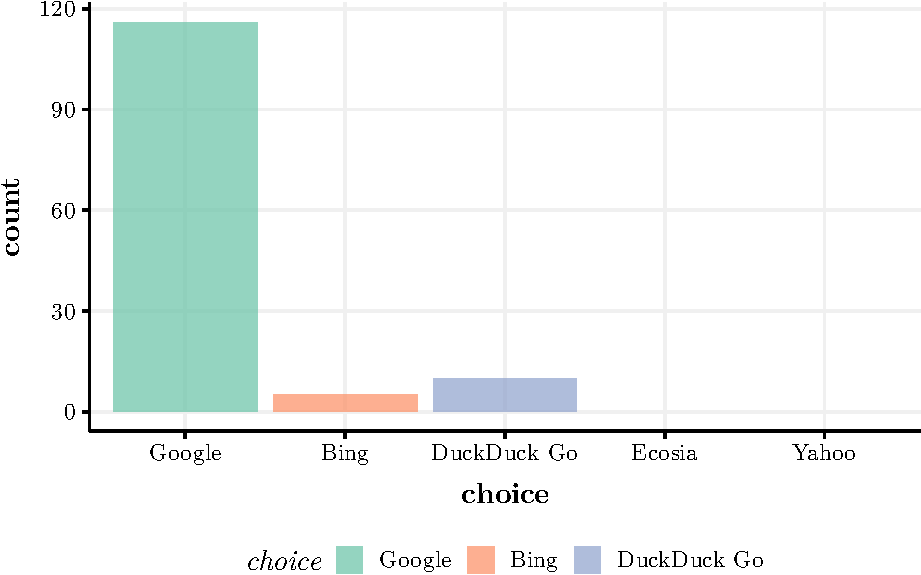
\includegraphics[width=0.8\textwidth]{Results-July19_files/figure-latex/choice_se-1} \end{center}

\hypertarget{creates-dfs-for-comparison-pada-vs-pac}{%
\subsection{creates dfs for comparison pA\textbar D(A) vs pA\textbar C}\label{creates-dfs-for-comparison-pada-vs-pac}}

Mind there are two ways to operationalize the effect:

\begin{enumerate}
\def\labelenumi{\arabic{enumi})}
\item
  compared with choice-screen
\item
  compared with any other default
\end{enumerate}

\hypertarget{creates-df-for-default-condition}{%
\subsection{creates df for default condition}\label{creates-df-for-default-condition}}

\hypertarget{status-quo-effects-search}{%
\section{Status Quo Effects Search}\label{status-quo-effects-search}}

\hypertarget{bing}{%
\subsection{Bing}\label{bing}}

*Interesting. Status quo effect goes down. People start switching. I need longer questionnaire. Hopefully, 5 enough. If not, run final version with 7 questions? Not sure it's worth it

*Different comparison: Pb\textbar B compared with any other default

Now, do the same for Q5

See how this effect affects Google

\hypertarget{video-had-no-effect.-probably-everyone-pais-attention.-check-number-of-correct-answers}{%
\subsection{Video had no effect. Probably everyone pais attention. Check number of correct answers}\label{video-had-no-effect.-probably-everyone-pais-attention.-check-number-of-correct-answers}}

See if video had an effect\ldots{} It did not work out. No difference

Substantial effect! lowers use of Google!

\hypertarget{yahoo}{%
\subsection{Yahoo}\label{yahoo}}

Check status quo effects for Yahoo. There is no variance, so just report counts

\hypertarget{duckduck-go}{%
\subsection{DuckDuck Go}\label{duckduck-go}}

Do the same with DuckDuckGo

Compare with other defaults. Do chi-squared test.

\hypertarget{big-regression-general-analysis-status-quo-effect}{%
\subsection{Big regression general analysis status quo effect}\label{big-regression-general-analysis-status-quo-effect}}

There si something wrong with the default data set. Showing NAs in assigned to a

Data defaults without Google

Interesting coefficients, qualitatively. Now, run glm because p\textgreater1

\hypertarget{check-if-those-who-use-the-default-use-another-one-too}{%
\subsection{Check if those who use the default use another one too!}\label{check-if-those-who-use-the-default-use-another-one-too}}

This is important. q1 only a few use more than one, q3 many more explore.

Code below irrelevant. q1 only one person used more than one

Code above is not what I need. The relevant variable is stat\_quo\_qi * just\_one\_qi

\hypertarget{now-with-the-second-experiment}{%
\subsubsection{Now with the second experiment}\label{now-with-the-second-experiment}}

Interesting result. More people tend to use Bing exclusively over time.

\hypertarget{results-weather-apps}{%
\section{Results Weather Apps}\label{results-weather-apps}}

One plot for sq q1 for each (a1\_q1, a2\_q1, a3\_q1)

Another for sq q3 for each (a1\_q3, a2\_q3, a3\_q3)

Effect\_plot to show correlations browsers/s.engines controlling for changes in OSX market shares

\hypertarget{appendix}{%
\section{Appendix}\label{appendix}}

\begin{table}[!htbp] \centering \renewcommand*{\arraystretch}{1.1}\caption{Summary Statistics}\resizebox{\textwidth}{!}{
\begin{tabular}{lrrrrrrl}
\hline
\hline
choice\_search & \multicolumn{3}{c}{0} & \multicolumn{3}{c}{1} &   \\ 
 Variable & \multicolumn{1}{c}{N} & \multicolumn{1}{c}{Mean} & \multicolumn{1}{c}{SD} & \multicolumn{1}{c}{N} & \multicolumn{1}{c}{Mean} & \multicolumn{1}{c}{SD} & \multicolumn{1}{c}{Test} \\ 
\hline
age & 126 & 38 & 12 & 131 & 37 & 13 & F$=0.604^{}$ \\ 
education & 126 &  &  & 131 &  &  & X2$=2.313^{}$ \\ 
... college degree & 45 & 36\% &  & 57 & 44\% &  &  \\ 
... graduate degree & 24 & 19\% &  & 19 & 15\% &  &  \\ 
... high school & 19 & 15\% &  & 20 & 15\% &  &  \\ 
... some college & 36 & 29\% &  & 34 & 26\% &  &  \\ 
... some high-school & 2 & 2\% &  & 1 & 1\% &  &  \\ 
computer\_use & 126 &  &  & 131 &  &  & X2$=5.285^{}$ \\ 
... between 2-4 hours/day & 24 & 19\% &  & 29 & 22\% &  &  \\ 
... between 4-6 hours/day & 31 & 25\% &  & 20 & 15\% &  &  \\ 
... between 6-8 hours/day & 27 & 21\% &  & 30 & 23\% &  &  \\ 
... more than 8 hours/day & 41 & 33\% &  & 44 & 34\% &  &  \\ 
... up to 2 hours/day & 3 & 2\% &  & 8 & 6\% &  &  \\ 
gender & 126 &  &  & 131 &  &  & X2$=1.793^{}$ \\ 
... female & 57 & 45\% &  & 66 & 50\% &  &  \\ 
... male & 65 & 52\% &  & 63 & 48\% &  &  \\ 
... non-binary & 3 & 2\% &  & 2 & 2\% &  &  \\ 
... prefer not to say & 1 & 1\% &  & 0 & 0\% &  &  \\ 
ethnicity & 126 &  &  & 131 &  &  & X2$=2.246^{}$ \\ 
... african american & 13 & 10\% &  & 8 & 6\% &  &  \\ 
... american indian & 12 & 10\% &  & 12 & 9\% &  &  \\ 
... asian & 1 & 1\% &  & 1 & 1\% &  &  \\ 
... hispanic & 10 & 8\% &  & 9 & 7\% &  &  \\ 
... other & 2 & 2\% &  & 1 & 1\% &  &  \\ 
... white & 88 & 70\% &  & 100 & 76\% &  & \\ 
\hline
\hline
\multicolumn{8}{l}{Statistical significance markers: * p<0.1; ** p<0.05; *** p<0.01}\\ 
\end{tabular}
}
\end{table}

\begin{table}[!htbp] \centering \renewcommand*{\arraystretch}{1.1}\caption{Summary Statistics}\resizebox{\textwidth}{!}{
\begin{tabular}{lrrrrrrl}
\hline
\hline
Bing\_default & \multicolumn{3}{c}{0} & \multicolumn{3}{c}{1} &   \\ 
 Variable & \multicolumn{1}{c}{N} & \multicolumn{1}{c}{Mean} & \multicolumn{1}{c}{SD} & \multicolumn{1}{c}{N} & \multicolumn{1}{c}{Mean} & \multicolumn{1}{c}{SD} & \multicolumn{1}{c}{Test} \\ 
\hline
age & 162 & 44 & 14 & 157 & 42 & 15 & F$=1.195^{}$ \\ 
education & 162 &  &  & 157 &  &  & X2$=3.527^{}$ \\ 
... college degree & 70 & 43\% &  & 68 & 43\% &  &  \\ 
... graduate degree & 29 & 18\% &  & 32 & 20\% &  &  \\ 
... high school & 17 & 10\% &  & 23 & 15\% &  &  \\ 
... some college & 45 & 28\% &  & 32 & 20\% &  &  \\ 
... some high-school & 1 & 1\% &  & 2 & 1\% &  &  \\ 
computer\_use & 162 &  &  & 157 &  &  & X2$=2.036^{}$ \\ 
... between 2-4 hours/day & 23 & 14\% &  & 30 & 19\% &  &  \\ 
... between 4-6 hours/day & 38 & 23\% &  & 31 & 20\% &  &  \\ 
... between 6-8 hours/day & 46 & 28\% &  & 41 & 26\% &  &  \\ 
... more than 8 hours/day & 42 & 26\% &  & 40 & 25\% &  &  \\ 
... up to 2 hours/day & 13 & 8\% &  & 15 & 10\% &  &  \\ 
gender & 162 &  &  & 157 &  &  & X2$=0.793^{}$ \\ 
... female & 79 & 49\% &  & 72 & 46\% &  &  \\ 
... male & 76 & 47\% &  & 80 & 51\% &  &  \\ 
... non-binary & 5 & 3\% &  & 4 & 3\% &  &  \\ 
... prefer not to say & 2 & 1\% &  & 1 & 1\% &  & \\ 
\hline
\hline
\multicolumn{8}{l}{Statistical significance markers: * p<0.1; ** p<0.05; *** p<0.01}\\ 
\end{tabular}
}
\end{table}

\end{document}
